\documentclass[11pt]{article}
\title{CS 5114: Theory of Algorithms}
\nonstopmode
%\usepackage[utf-8]{inputenc}
\usepackage{graphicx} % Required for including pictures
\usepackage[figurename=Figure]{caption}
\usepackage{float}    % For tables and other floats
\usepackage{verbatim} % For comments and other
\usepackage{amsmath}  % For math
\usepackage{amssymb}  % For more math
\usepackage{amsthm}  % For theorems and proofs
\usepackage{mathtools}
\usepackage{fullpage} % Set margins and place page numbers at bottom center
\usepackage{paralist} % paragraph spacing
\usepackage{listings} % For source code
\usepackage{subfig}   % For subfigures
\usepackage{sectsty}
\usepackage[super]{nth}
%\usepackage{physics}  % for simplified dv, and
\usepackage{enumitem} % useful for itemization
\usepackage{siunitx}  % standardization of si units
\usepackage{breqn}
\usepackage{chngcntr}
\usepackage{setspace}
\usepackage{multicol}
\usepackage{bookmark}
\usepackage{listings}
\usepackage{color}
\usepackage{hyperref}
\usepackage{titlesec}
\usepackage[linesnumbered, ruled, vlined, commentsnumbered]{algorithm2e}

\setlength{\parskip}{0pt}
\raggedcolumns


\titleformat*{\section}{\normalsize\bfseries}
\titleformat*{\subsection}{\normalsize\bfseries}
\titleformat*{\subsubsection}{\normalsize\bfseries}
\titleformat*{\paragraph}{\normalsize\bfseries}


\begin{document}
\bibliographystyle{ieeetr}

\begin{center}
	\hrule
	\vspace{.4cm}
	{\textbf { \large Bin Packing Problem using Greedy Algorithms}}
\end{center}
\textbf{Name:}\ Matthew Trang \hspace{\fill} \textbf{Date:} \today \\
{ \textbf{Student PID:}} \ mattluutrang \hspace{\fill} \textbf{Project: } 2
\vspace{.4cm}
\hrule

% \section*{Abstract}
% The optimization problem in this project is the Bin Packing Problem. The Bin Packing Problem is a
% problem in which items are packed into bins of a certain capacity. The goal is to pack the items
% into the fewest number of bins. Each item has a corresponding weight, which is less than the bins
% capacity. In this project, we will implement two greedy algorithms to solve the Bin Packing Problem,
% and compare and contrast their performance with respect to optimality, run time, and asymptotic
% complexity. We will also compare the algorithms to a brute force algorithm.

\section{Optimization Problem and Description}
In this problem, we are given ${n}$ items of different weights and bins each with capacity ${c}$,
with the restriction that all weights must be less than or equal to ${c}$. The list of items is
given sequentially, thus cannot be sorted beforehand, and the items are not necessarily in any
order. The goal is to place all the items in bins to minimize the amount of bins that are needed to
hold all of the items. This situation holds real world parallels to numerous logistics problems, such as loading
shipping containers, or transportation of luggage at an airport.
\subsection{Input Parameters}
The input to the problem is a list of ${n}$ objects of different weights. The additional parameter
for the problem is the capacity of the bins, ${c}$. The inputs are considered in a sequential order,
which limits the ability to sort the input list.

\subsection{Objective Function}
The objective function for the problem can be written as the following minimization of the number of
bins, ${B}$, that are needed to hold all of the items. Given a finite set of ${O}$ objects, a bin
capacity ${c}$, and a
weight ${w_o \leq c}$ for each ${o \in O}$,

\begin{equation}
	\text{minimize } B  = \sum_{i=1}^{n} y_i
\end{equation}
where, ${y_i}$ is an indicator variable, ${y_i = 1}$ if the bin ${i}$ is used. \\
While the exact number for the optimal solution would require solving the optimization problem, we
are able to formulate a lower-bound approximation for the number of bins used by taking the sum of
all objects and dividing by the bin capacity, ${c}$, or
\begin{equation}
	\lim_{B} \geq \lceil \sum_{i=1}^{n} w_i / c \rceil
\end{equation}
\subsection{Expected Outputs}
The expected output of the algorithm is the number of bins needed to pack all the objects.
For example, when given the input weights of ${{4, 8, 1, 2, 4, 1}}$ and a bin capacity of
${10}$,
the algorithm should output 2 bins, as one form of the optimal solution would place the items into bins of
${[8,2], [4,4,1,1]}$.

\subsection{Large Size Challenges}
The problem is an NP hard problem, as in order to find the global optimum, we need to consider
every combination of objects within bins. Thus, finding the exact minimum number of bins takes
factorial time. Therefore, given a large enough input, finding the optimal solution could be almost
impossible to calculate.

\section{Greedy Algorithms}
\subsubsection{First Greedy Algorithm}
The first algorithm for the problem uses an idea of greedily selecting the spot which it fits best
in, where the heuristic for best is in terms of the remaining space in the bin. In other words, if an
object could fit into two different bins, it would chose the bin that has the least space remaining.
In the algorithm, we start with an input array of weights for the objects, ${O}$, and a bin
capacity, ${c}$. Then, we create an array of initially empty bins, ${B}$, and set our number of bins
used currently to 0. We iterate through each object, and for each iteration step, we check all of
the currently used bins to see which one the object will fit in best. If the object does fit in any
one bin, then
the space taken up by the object is added to that heuristically selected bin. Otherwise, we put the
item into a new bin and increment the number of bins used.

\begin{algorithm}[H]
	\SetAlgoLined
	\SetStartEndCondition{ }{}{}%
	\SetKwProg{Fn}{def}{\string:}{}
	\SetKwFunction{Range}{range}%%
	\SetKw{KwTo}{in}\SetKwFor{For}{for}{\string:}{}%
	\SetKwIF{If}{ElseIf}{Else}{if}{:}{elif}{else:}{}%
	\SetKwFor{While}{while}{:}{fintq}%
	\AlgoDontDisplayBlockMarkers\SetAlgoNoEnd\SetAlgoNoLine%
	\KwData{${O}$ is an array of object costs, ${c}$ is the capacity of the bins, and ${n}$ is the number of objects}%
	\KwResult{the number of bins needed to pack all the objects}%
	\Begin{
		total $\leftarrow$ 0 \\
		initialize the array of bins to be empty \\
		\For{obj in O}{
			rem ${\leftarrow  c + 1}$ \\
			idx ${\leftarrow}$  0 \\
			\For{j in range total}{
				\If{obj ${\leq}$ bins[j] and bins[j] - obj ${<}$  rem}{
					rem ${\leftarrow}$  bins[j] + O[object] \\
					idx ${\leftarrow}$ j
				}
			}
			\If{${c + 1 == rem}$ }{
				bins[total] ${\leftarrow}$  c - obj \\
				total ${\leftarrow}$ total + 1 \\
			}
			\Else( if it fits){
				bins[idx] ${\leftarrow}$ bins[idx] - obj \\
			}
		}
		\Return{total}
	}
	\caption{Greedy 1(${O}$, ${c}$, ${n}$)\label{greedy1}}
\end{algorithm}

This first greedy algorithm has a time complexity of ${O(n^2)}$, where ${n}$ is the number of
objects. The first for loop iterates through each object, and the asymptotic behavior of the
algorithm occurs where each object takes its own bin, resulting in the second iteration over the
number of bins to also be an iteration of the number of objects. The other operations in the
algorithm are all of constant time. The space complexity of the algorithm is linear, as the
algorithm has to initialize the array of bins to be empty using the worst case size of the bins,
which would be ${n}$ bins.
% This algorithm able to reach an ${\sqrt{2}}$-approximation of the optimal
% solution of bins used, which can be calculated using Equation 2, meaning at most, the algorithm will
% use approximately 1.7 times the optimal number of bins \cite{noauthor_bin_2016}.


\subsubsection{Second Greedy Algorithm}
The second algorithm uses the idea of greedily selecting the spot which was last used to store an
object in to store the next object as well. This algorithm is simpler than the first algorithm, but
runs in linear time. The algorithm also is able to compute the local optimal bin number without the
use of additional allocated space for an array of bins, thus achieving constant space complexity.
The algorithm first begins with a count of the total used bins initialized to 0 and a remainder
variable set to the capacity of the bins. Then the algorithm iterates through the objects, and for
each object, if the object fits in the remaining space in the bin, then the remaining space variable
is decremented by the weight of the object. If the object does not fit in the remaining space, then
a new bin is created, and the remaining space is set to the value of the capacity minus that of the
object which was just placed.

\begin{algorithm}[H]
	\SetAlgoLined
	\SetStartEndCondition{ }{}{}%
	\SetKwProg{Fn}{def}{\string:}{}
	\SetKwFunction{Range}{range}%%
	\SetKw{KwTo}{in}\SetKwFor{For}{for}{\string:}{}%
	\SetKwIF{If}{ElseIf}{Else}{if}{:}{elif}{else:}{}%
	\SetKwFor{While}{while}{:}{fintq}%
	\AlgoDontDisplayBlockMarkers\SetAlgoNoEnd\SetAlgoNoLine%
	\KwData{${O}$ is a array of object costs, ${c}$ is the capacity of the bins, and ${n}$ is the number of objects}%
	\KwResult{the number of bins needed to pack all the objects}%
	\Begin{
		$total \leftarrow$ 0 \\
		rem $\leftarrow$ ${c}$  \\
		\For{obj in ${O}$ }{
			\If{${obj \leq rem}$ }{
				rem $\leftarrow$ rem - obj \\
			}
			\Else( if it doesn't fit){
				total $\leftarrow$ total + 1 \\
				rem $\leftarrow$ c - obj  \\
			}
		}
	}
	\caption{Greedy 2(${O}$, ${c}$, ${n}$)\label{greedy2}}
\end{algorithm}

The second greedy algorithm has a time complexity of ${O(n)}$, where ${n}$ is the number of objects.
Due to the fact that the algorithm merely checks if it can fit in the previous bin, and not in any
of the preceding bins, the algorithm only iterates through the objects once. The space complexity is
also impacted by this, as there is no longer a need to store an array of ${n}$ bins, and instead a
single remaining capacity variable can be used. However, the optimality of this algorithm is
significantly worse than that of the first greedy algorithm, as the bins which are passed over could
have potentially been filled by another object.
% This version of the algorithm is a 2-approximation
% of the optimal value, thus, its upper bound of the predicted minimum is at most 2 times that of the
% optimal value from equation 2 \cite{noauthor_bin_2016}.

% \subsubsection{Brute Force Algorithm}
% The brute force implementation of the algorithm computes the number of bins needed for every single
% combination of items within a bin. This is done by taking all the possible permutations of the
% objects, and then finding the number of bins needed for each permutation using a next fit
% philosophy. Then, after iterating through every possible permutation, the algorithm returns the
% minimum value that it had achieved. This algorithm is capable of finding the exact optimal solution
% for the problem. However, the time complexity for the algorithm is ${O(n!)}$, thus is not feasible
% for problems of large size. The algorithm was unable to be tested after reaching an ${n}$ of 13, as
% it took too long to run.

\section{Comparative Performance Analysis}

\subsection{Experimental Results - Small-size}
\begin{figure}[H]
	\centering
	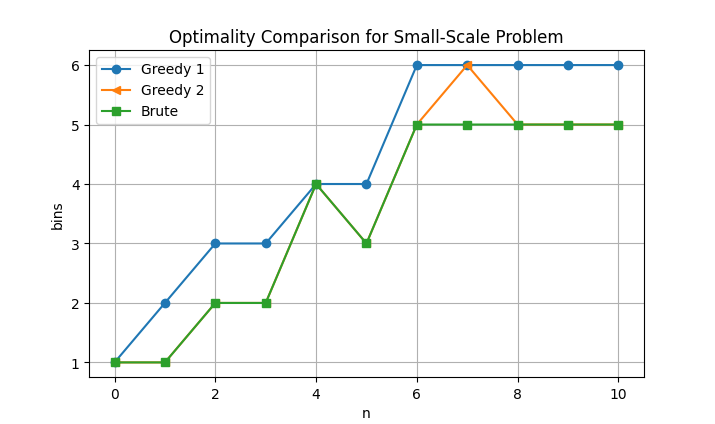
\includegraphics[width=0.5\textwidth]{images/smallscale_optimality.png}
	%\caption{caption\label{smallscale_optimality}}
\end{figure}
\begin{figure}[H]
	\centering
	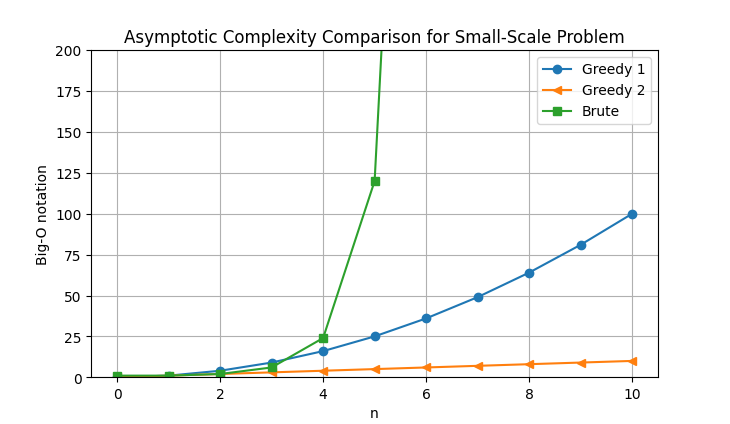
\includegraphics[width=0.5\textwidth]{images/smallscale_complexity.png}
	%\caption{caption\label{smallscale_complexity}}
\end{figure}
\begin{figure}[H]
	\centering
	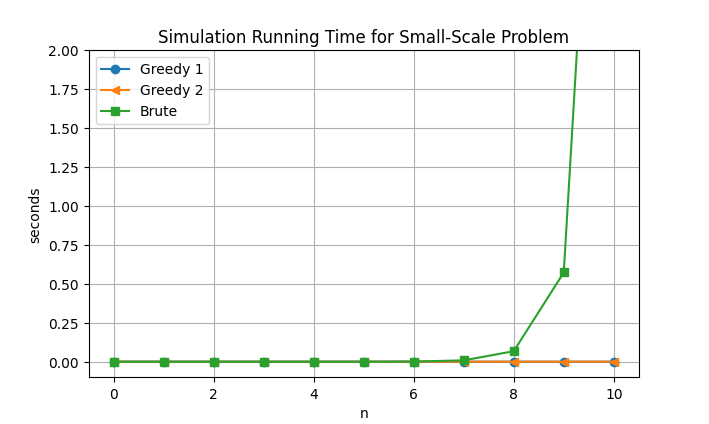
\includegraphics[width=0.5\textwidth]{images/smallscale_simtime.png}
	%\caption{caption\label{smallscale_simtime}}
\end{figure}

\subsection{Small-size Results Analysis}
In the small-size experimental results, the number of bins that each algorithm used for the problem
size ${n}$ was compared. As expected, the green brute force method had the lowest number of bins
across all ${n}$, as it achieves the optimal value. The first greedy algorithm unexpectedly performs
worse than the second greedy algorithm, which is likely due to the fact that at a small problem
size, there are less remaining objects that are able to perfectly fit the size of a leftover bin.

For the asymptotic complexity, the first greedy algorithm has a complexity of ${O(n^2)}$, while the
other greedy algorithm is able to execute in ${O({n})}$ time, and the brute force algorithm is the
worst with ${O(n!)}$ time. The simulation running time for the different algorithms also reflects
this.

\subsection{Experimental Results - Large-size}
\begin{figure}[H]
	\centering
	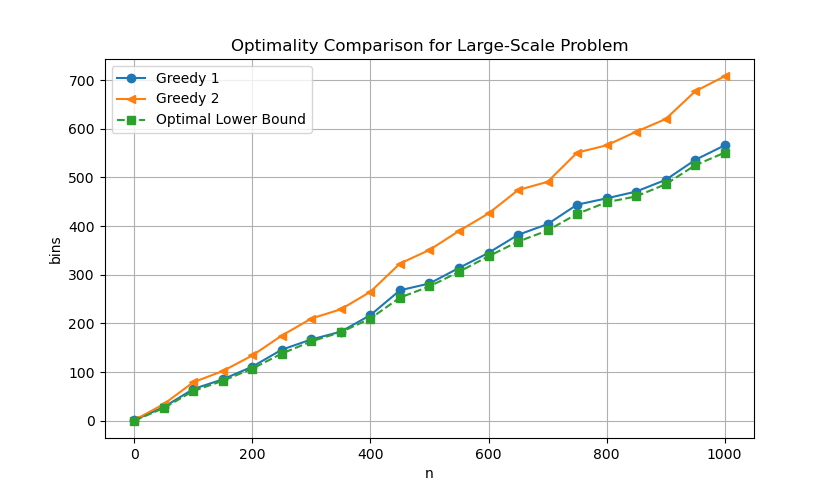
\includegraphics[width=0.5\textwidth]{images/largescale_optimality.png}
	%\caption{caption\label{largescale_optimality}}
\end{figure}
\begin{figure}[H]
	\centering
	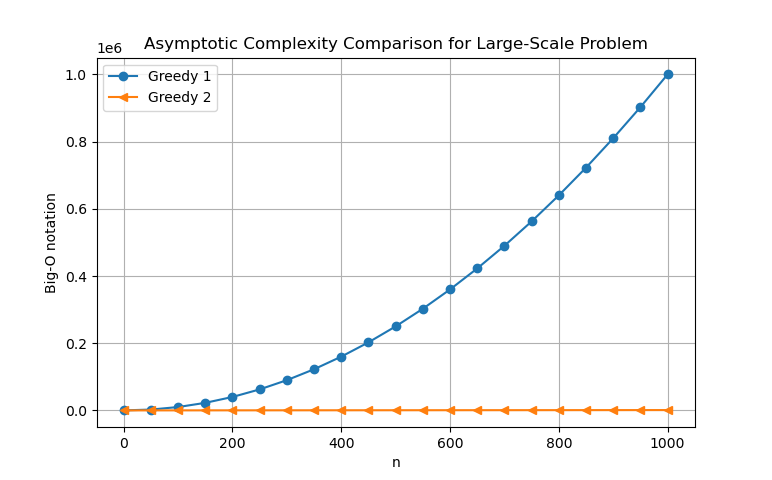
\includegraphics[width=0.5\textwidth]{images/largescale_complexity.png}
	%\caption{caption\label{largescale_complexity}}
\end{figure}
\begin{figure}[H]
	\centering
	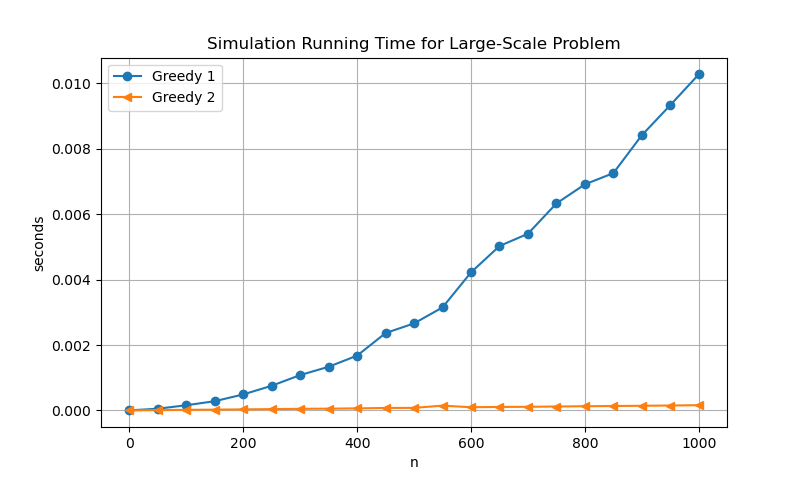
\includegraphics[width=0.5\textwidth]{images/largescale_simtime.png}
	%\caption{caption\label{largescale_simtime}}
\end{figure}

\subsection{Large-size Results Analysis}
In the large-size experimental results, it can be seen that the first greedy algorithm performs
much closer to that of the theoretical optimal lower bound compared to that of the second greedy
algorithm. As the value for ${n}$ increases, the difference between greedy 1 and greedy 2
increases. Theoretically, as the limit of ${n}$ approaches infinity, the algorithms will
approach their true approximate optimal values.

For the asymptotic complexity, the first greedy algorithm has a complexity of ${O(n^2)}$, while the
other greedy algorithm is able to execute in ${O({n})}$ time, and the simulation time of the
programs reflect this.

\section{Parameters and Extensions}
\subsection{Parameter 1 - Capacity}
In this section we first explore the effect of capacity of the bins. In the previous tests, our
capacity was 10. For these parameter tests, we compare the results of capacities of 10, 500, and
1000.
\begin{figure}[H]
	\centering
	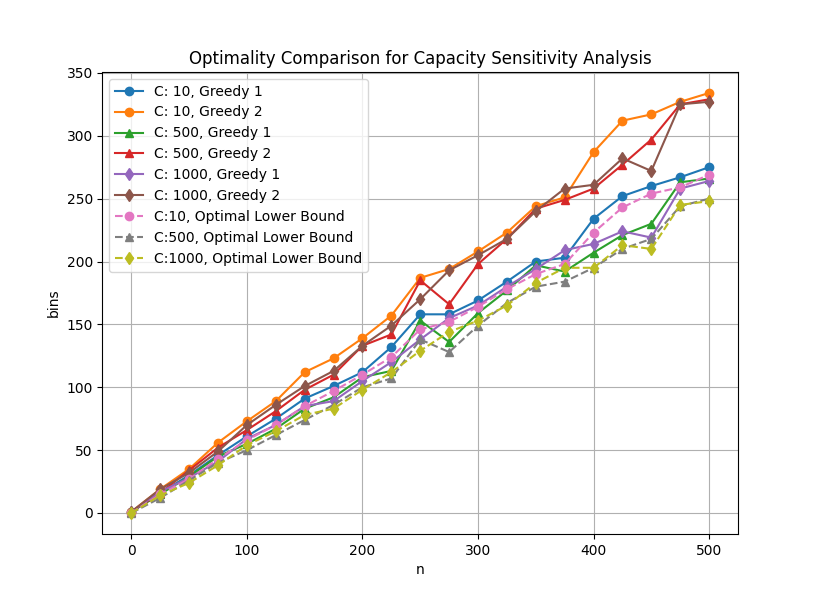
\includegraphics[width=0.5\textwidth]{images/s1_optimality.png}
	%\caption{\label{fig:sample}}
\end{figure}
\begin{figure}[H]
	\centering
	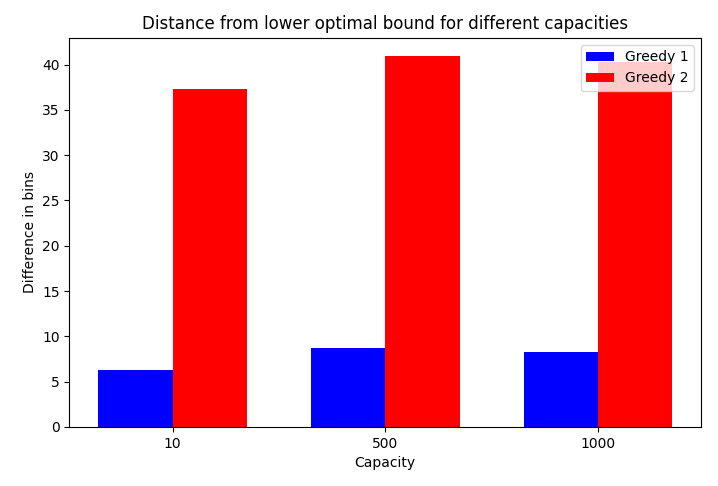
\includegraphics[width=0.45\textwidth]{images/s1_optdiff.png}
	%\caption{\label{fig:sample}}
\end{figure}
\begin{figure}[H]
	\centering
	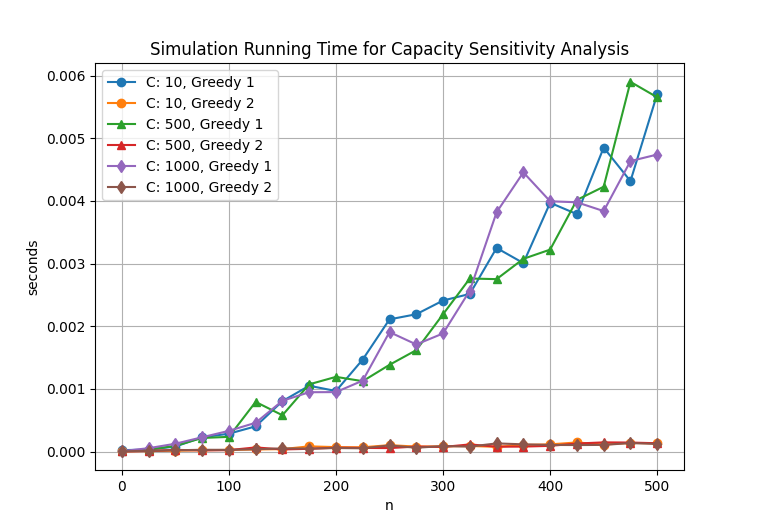
\includegraphics[width=0.5\textwidth]{images/s1_simtime.png}
	%\caption{\label{fig:sample}}
\end{figure}
\begin{figure}[H]
	\centering
	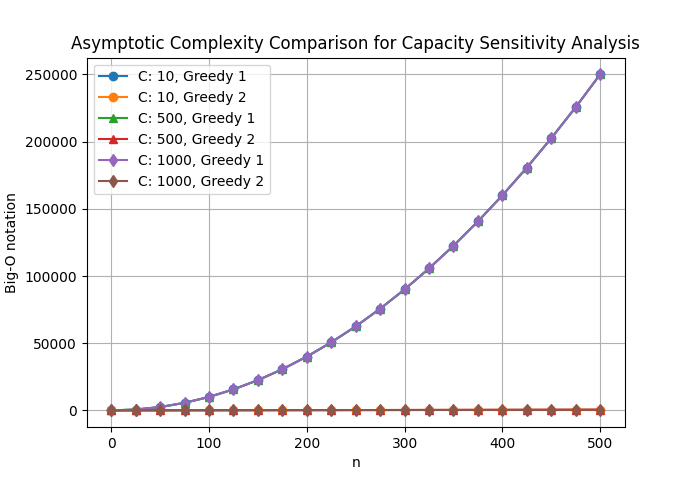
\includegraphics[width=0.5\textwidth]{images/s1_complexity.png}
	%\caption{\label{fig:sample}}
\end{figure}
The change in capacity can be seen to be insignificant with respect to run time and complexity.
This is likely because the capacity of the bins is not important for the runtime of the
algorithm, and the complexities are still limited by the number of objects. However, there is a
noticeable difference in terms of optimality, likely because with a larger capacity, the
deviation of the weights of the generated objects increases, and it is slightly less likely that
the objects will fit as optimally.

\subsection{Parameter 2 - Sorted Input}
In this section we first explore the effect of sorting the array of objects before passing the
array to the algorithms. The arrays were sorted in decreasing order of their weights, and
nothing was changed in either algorithm.
\begin{figure}[H]
	\centering
	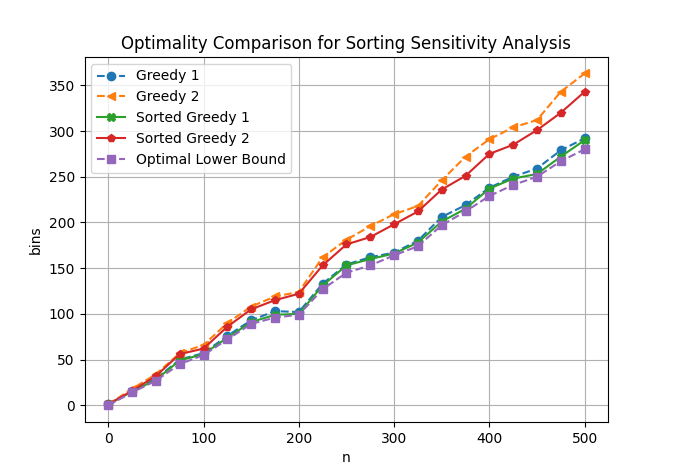
\includegraphics[width=0.5\textwidth]{images/s2_optimality.png}
	%\caption{\label{fig:sample}}
\end{figure}
\begin{figure}[H]
	\centering
	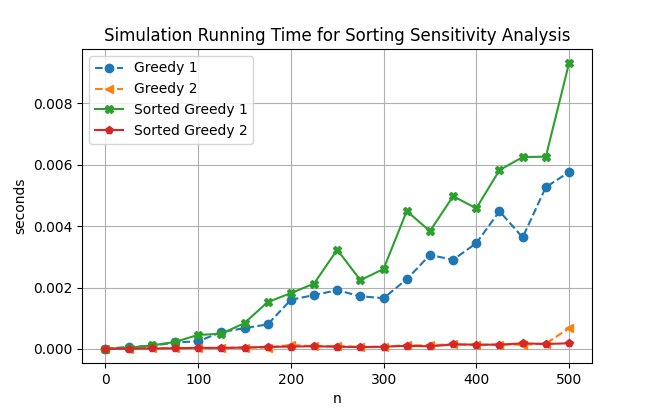
\includegraphics[width=0.5\textwidth]{images/s2_simtime.png}
	%\caption{\label{fig:sample}}
\end{figure}
\begin{figure}[H]
	\centering
	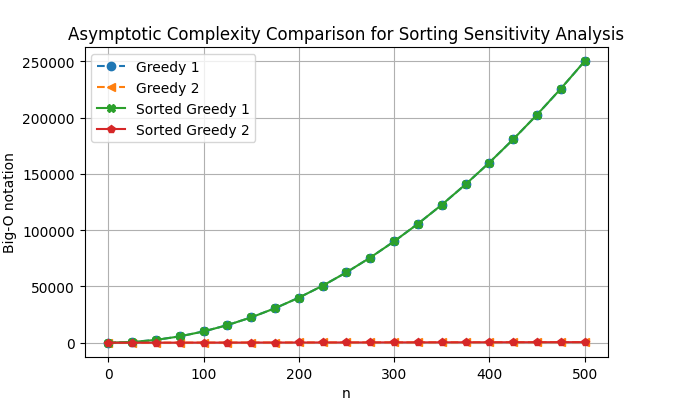
\includegraphics[width=0.5\textwidth]{images/s2_complexity.png}
	%\caption{\label{fig:sample}}
\end{figure}
The sorted input did not affect the complexity of the algorithms, as the sorting was
not considered part of the algorithm, therefore the asymptotic behavior of the algorithms did not change. It did however cause an increase in the simulation
runtime for algorithm 1, and also a decrease in the amount of bins that both algorithms ended up using. The
improvement in the optimality for the first algorithm makes sense, as the decreasing weights
ensures that we are placing the smallest objects when there is the least space available.
Similarly, for the second algorithm, once we reach the smallest objects, the sequential objects
are more likely to also fit in the same bin, thus being more optimal. Run time increases for
algorithm 1 because we fill bins faster in the beginning, thus we have iterate through more bins
overall.




%\bibliography{AlgP2.bib}


\end{document}
